\documentclass{article}

\usepackage[printqrbox=false,printhint=false,printanswer=true,printmarkingguide=false,printdraftpaper=false]{unswalgos}

\usepackage{tikz}
\usetikzlibrary{patterns}
\usetikzlibrary{shapes,fit}
\usepackage{tkz-fct}
\usepackage{wrapfig}
\usepackage{subfig}

\usepackage{mathtools}
\usepackage{amssymb}
\usepackage{booktabs,multicol,multirow}
\usepackage{wasysym}
\usepackage{tcolorbox}

\DeclareMathOperator*{\argmax}{arg\,max}
\DeclareMathOperator*{\argmin}{arg\,min}
\DeclareMathOperator{\NAND}{NAND}
\DeclareMathOperator{\AND}{AND}
\DeclareMathOperator{\OR}{OR}
\DeclareMathOperator{\NOT}{NOT}

\usepackage{xspace}

\fancyfoot[L]{\leftmark}
\fancyfoot[R]{\rightmark}

\usepackage{graphicx}
\usepackage{float}
\usepackage{subfigure}

\usepackage{framed}
% This enables new paragraphs without indentation
\usepackage[parfill]{parskip}

\newcommand{\sem}{22T2}
\newcommand{\semester}{Term 2, 2022}
\SubjectNo{COMP3151}
\newcommand{\taskname}{Homework 3}
\Institution{Jinghan Wang, z5286124} % Replace this with your name and zID


\begin{document}
\begin{Question} [\large\textbf {Manna-Pnueli Algorithm {[2 marks]}}]
Recall the Manna-Pnueli algorithm from Lecture 3.
\begin{figure}[H]
    \centering 
    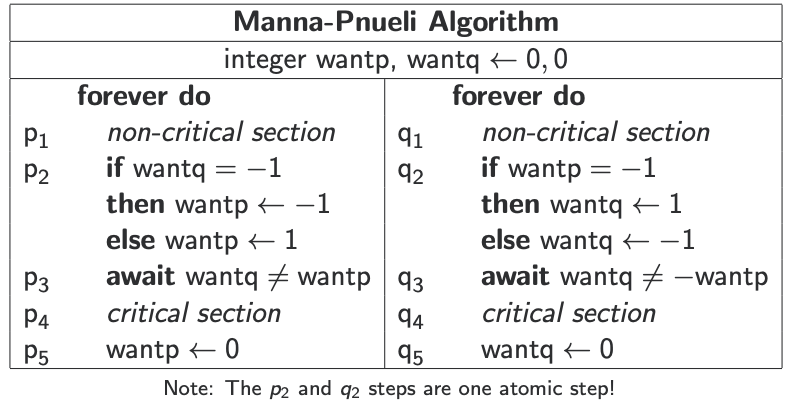
\includegraphics[width=0.8\textwidth]{DV_demand1}
\end{figure}
Recall that the if condition and body must be executed as one atomic step. If this were not the case, find an interleaving that violates mutual exclusion. That is, split the if condition into two steps (condition and body) and find an execution such that both processes end up in their critical section simultaneously.\\

\begin{answer}
Answer: \\
\begin{quote}
    
\end{quote}
\end{answer}
\end{Question}

\clearpage
\begin{Question} [\large\textbf {Szymanski's Algorithm {[5 marks]}}]
In this Promela code archive you will find a Promela model of Szymanski's algorithm for three processes, broken down to satisfy LCR, with a particular choice of test order for the various await statements. This choice happens to satisfy mutual exclusion and eventual entry (as you may check in Spin), but as mentioned in the lectures, not all choices do.\\\\
The task here is to twiddle with the test orders and figure out which orderings break the algorithm and which don't. You don't need to test all permutations, but do answer these questions:\\\\
Can you find any reorderings that break mutual exclusion and/or eventual entry? (You should be able to find at least one). Are there any awaits that don't seem sensitive to reordering at all? What if you reorder the tests for all the awaits in the exact same way? And finally, based on any error trails you obtain, can you form an educated guess about why the test order matters?\\\\
Explain your findings, informally and in your own words.\\\\

\begin{answer}
Answer: \\
\begin{quote}
    
\end{quote}
\end{answer}
\end{Question}

\clearpage
\begin{Question} [\large\textbf {Composing Solutions {[5 marks]}}]
Let $A$ and $B$ be two algorithms purported to solve the mutual exclusion problem for two processes. Let $C$ be the algorithm obtained by replacing the critical section of $A$ with the algorithm $B$:

\begin{figure}[H]
    \centering 
    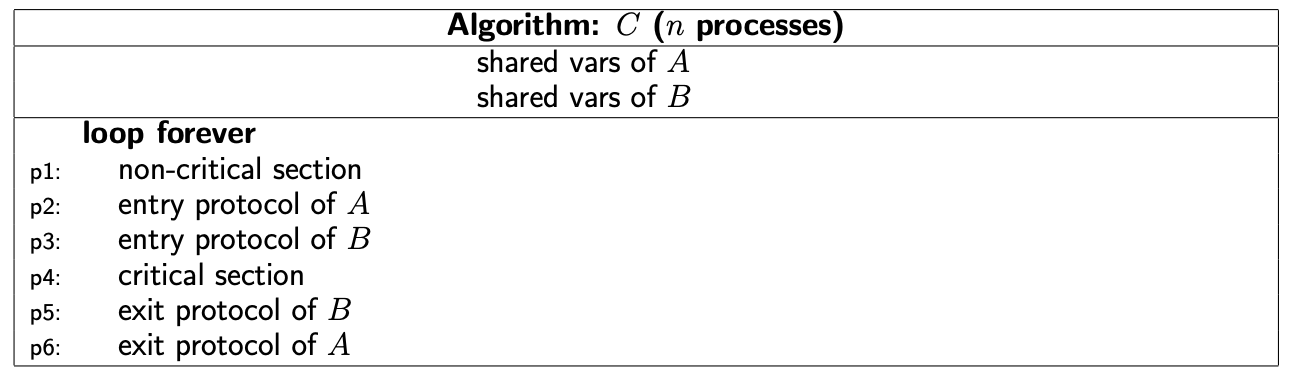
\includegraphics[width=0.8\textwidth]{DV_demand2}
\end{figure}
Assume that the shared variables of $A$ are disjoint from those of $B$. Are the following statements correct? Justify your answers with $1-2$ sentences.

$a)$ If either $A$ or $B$ satisfies mutual exclusion, then $C$ satisfies mutual exclusion.\\
$b)$ If $A$ has no unnecessary delay and $B$ satisfies mutual exclusion then $C$ has no unnecessary delay.\\
$c)$ If $A$ satifies mutual exclusion and $B$ has no unnecessary delay then $C$ has no unnecessary delay.\\
$d)$ If $A$ is deadlock free and B guarantees eventual entry then $C$ guarantees eventual entry.\\

\begin{answer}
Answer: \\
\begin{quote}
    
\end{quote}
\end{answer}
\end{Question}
    
\end{document}